\documentclass[a4paper, 12pt]{article}
\usepackage[utf8]{inputenc}
\usepackage[english,russian]{babel}
\usepackage[warn]{mathtext}
\usepackage{graphicx}
\usepackage{float}
\usepackage{multirow}
\restylefloat{table}
\usepackage{amsmath}
\usepackage{floatflt}
\usepackage[T2A]{fontenc}
\usepackage[left=20mm, top=20mm, right=20mm, bottom=20mm, footskip=10mm]{geometry}

\tolerance 1414
\hbadness 1414
\emergencystretch 1.5em
\hfuzz 0.3pt        % размер максимального переполнения без warning'a
\widowpenalty=10000 % запрещает одиночную строку абзаца в начале страницы
\vfuzz \hfuzz
\raggedbottom       % если на странице мало содержимого, добавить пустое место в конце, а не в середине страницы



\begin{document}

\begin{titlepage}
	\centering
	\vspace{5cm}
	{\scshape\LARGE московский физико-технический институт (национальный исследовательский университет) \par}
	\vspace{6cm}
	{\scshape\Large Лабораторная работа 4.3.2 \par}
	{\huge\bfseries Дифракция света на ультразвуковых волнах \par}
	\vspace{1cm}
	\vfill
\begin{flushright}
	{\large Б03-102}\par
	\vspace{0.3cm}
	{\LARGE Куланов Александр}
\end{flushright}
	

	\vfill


	Долгопрудный, 2023 г.
\end{titlepage}

\begin{itemize}
	\item \textbf{Цель работы:} измерить координаты дифракционных полос, образующихся при дифракции света на акустической решетке, определить период этой решетки методом темного поля, рассчитать скорость ультразвука в воде
    \item \textbf{В работе используются:} оптическая скамья, осветитель, светофильтры, конденсор, щель, два длиннофокусных объектива, кювета с водой, кварцевый излучатель с микрометрическим винтом, генератор УЗ-частоты, частотомер, линза, отсчетное устройство, микроскоп.
\end{itemize}

\section{Экспериментальная установка}
\begin{figure}[H]
    \centering
    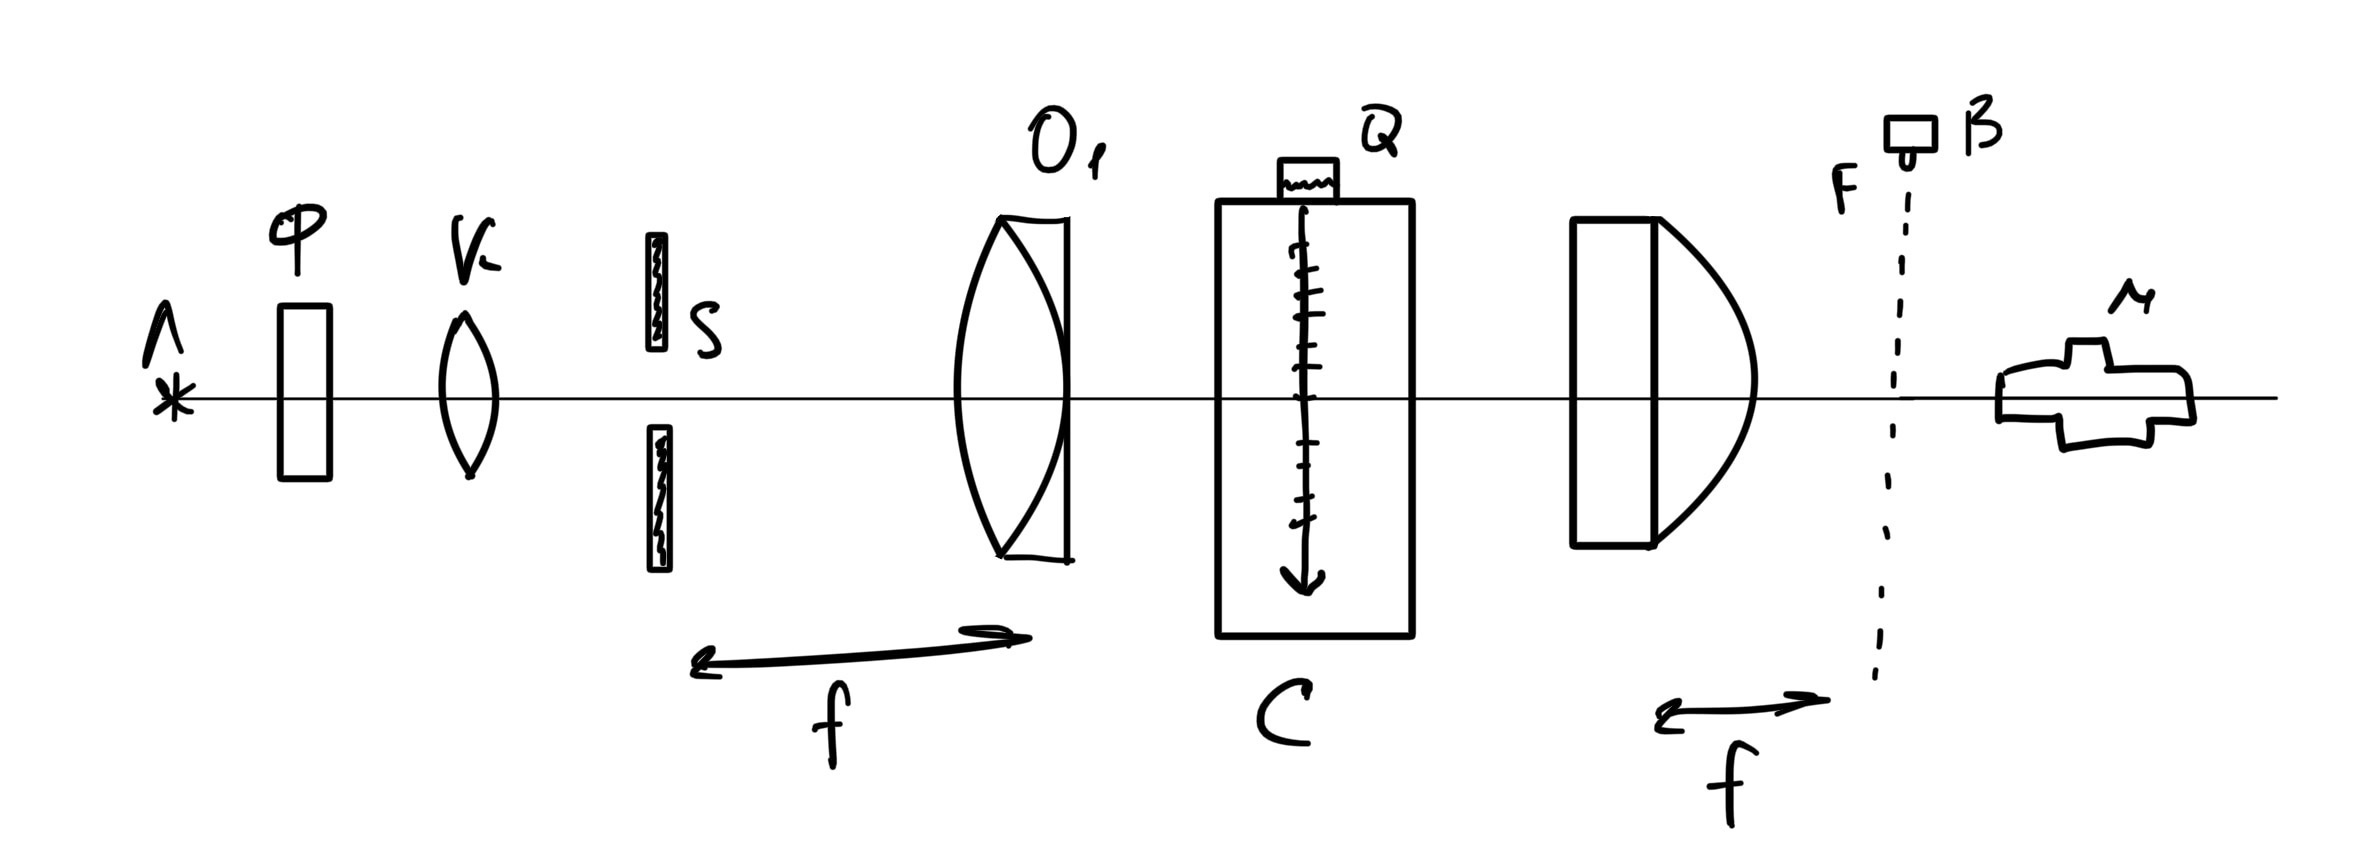
\includegraphics[width=1\textwidth]{set}
    \caption{Схема установки}
    \label{fig:set}
\end{figure}

Источник света Л через светофильтр Ф и конденсор К освещает щель $S$, которая расположена в фокусе объектива $\mathrm{O}_1$. Выходящий из объектива параллельный пучок света проходит через кювету $C$ перпендикулярно направлению распространения УЗ-волн. Эти волны возбуждаются в жидкости пьезокварцевой пластинкой $Q$, шрикреплённой к стенке кюветы. На кварцевую пластинку подаётся синусоидальное напряжение ультразвуковой частоты от генератора (на рис. 2 не показан). В результате взаимодействия света с ультразвуковой волной в фокальной плоскости второго объектива $\mathrm{O}_2$ образуется дифракционная картина, наблодаемая при помощи микроскопа М. При этом обязательно применяют монохроматическое излучение (красный светофильтр).

Дифракционные полосы ориентированы вертикально. Расстояние между ними можно измерить с помощью специального отсчётного устройства с микрометрическим винтом В. Этот винт передвигает размещённые на стекле отсчётного устройства тонкую реперную линию Рл, перекрестие $\Pi$ и толстую проволоку Пр, которая используется в методе тёмного поля. Все измерительные линии должны быть расположены в плоскости $F$ резкого изображения щели.

Чёткость дифракционньх полос зависит от ряда факторов, например, от ширины щели $S$, от её наклона по отношению к вертикали, от угла наклона кюветы к падающему лучу и т. д.
Длина $\Lambda$ ультразвуковой волны определяется по формуле
\begin{equation}
\Lambda \sin \Theta_m=m \lambda
\end{equation}
в силу малости углов $\Theta_m$ окончательное выражение может быть представлено в виде
\begin{equation}
l_m=m f \frac{\lambda}{\Lambda}
\end{equation}
где $l_m-$ измеренное на опыте линейное расстояние между $m$-м и нулевым максимумами, а $f$ - фокусное расстояние объектива $\mathrm{O}_2$.

Скорость $\nu$ распространения звука в воде можно рассчитать, если известна частота $\nu$ кварцевого излучателя:
\begin{equation}
v=\Lambda \nu
\end{equation}

\end{document}